% =====================================================================
%  Partie 3 — ACV et architecture
%  Les figures des diapositives sont signalées en commentaire « FIGURE ».
% =====================================================================
\part{ACV et architecture}

% ---------------------------------------------------------------------
\chapter{Méthode d'ACV de bâtiment}
\label{chap:methode-batiment}
\section{Indicateurs}

Dans le domaine du bâtiment, la norme EN 15804+A2 définit 13 indicateurs principaux :
\begin{itemize}
  \item changement climatique total, fossile, biogénique et lié à l'usage des terres (kg CO$_2$ éq.)
  \item appauvrissement de la couche d'ozone (kg CFC-11 éq.)
  \item acidification (mol H$^+$ éq.)
  \item eutrophisation des eaux douces (kg P éq.), marine (kg N éq.) et terrestre (mol N éq.)
  \item formation d'ozone photochimique (kg NMVOC éq.)
  \item épuisement des ressources minérales et métalliques (kg Sb éq.)
  \item épuisement des ressources fossiles (MJ)
  \item utilisation de l'eau (m$^3$ éq. de privation)
\end{itemize}

Aucune méthode d’agrégation n’est imposée réglementairement : actuellement, la RE 2020 n’exige qu’une ACV portant sur le seul changement climatique.

Notons qu'une solution qui réduit le carbone peut en dégrader d’autres : c’est ce qu’on appelle un transfert d’impact (par exemple, un isolant bas carbone mais plus consommateur). Pour s’en prémunir, l’architecte peut regarder au-delà du carbone, soit en choisissant lui-même quelques indicateurs pertinents pour son projet, soit en s’appuyant sur une méthode d’agrégation, en gardant à l’esprit ses hypothèses de pondération.

Pour aller plus loin : la méthode \emph{Environmental Footprint}\footfullcite{andreasibassi2023ef31}, développée par le Centre commun de recherche (JRC) de la Commission européenne, présente un intérêt particulier pour l'architecte : ses indicateurs sont ceux des FDES (voir partie suivante). Il est donc possible, à partir des valeurs disponibles sur la base INIES, d'appliquer ses facteurs de normalisation et de pondération pour obtenir un score environnemental unique, et ainsi comparer des variantes de projet au-delà du seul critère carbone. Le lecteur curieux pourra consulter le rapport de référence du JRC\footnote{\url{https://publications.jrc.ec.europa.eu/repository/handle/JRC130796}}. Il gardera à l'esprit que toute pondération repose sur des choix de valeurs : un score unique aide à décider, mais ne remplace pas l'examen des indicateurs détaillés.

\section{Modules}

Le cycle de vie d'un bâtiment est découpé en 4 modules (A, B, C et D), illustrés figure~\ref{fig:module}.
\begin{figure}[h]
    \centering
    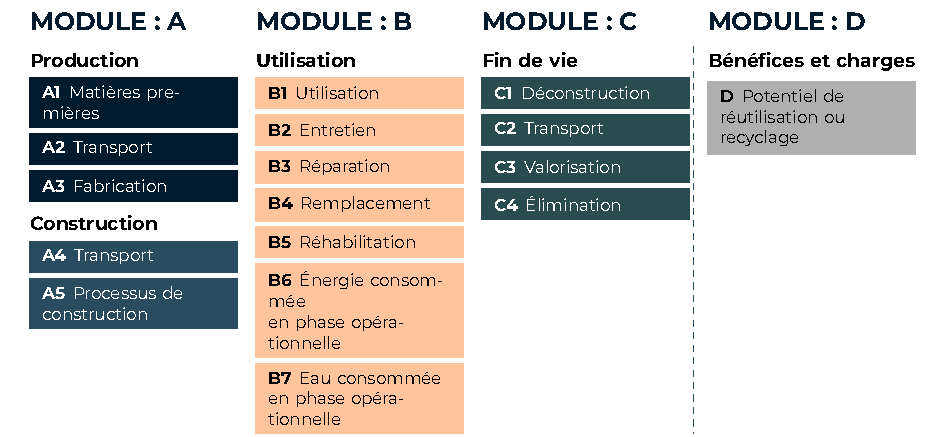
\includegraphics[width=1\linewidth]{figures/Modules.pdf}
    \caption{Modules de l'ACV de bâtiment}
    \label{fig:module}
\end{figure}

Les modules A couvrent l’amont et la construction. Les modules A1 à A3 correspondent à la production (ils incluent l’extraction des matières premières, le transport vers l’usine et la fabrication des produits). Les modules A4 et A5 correspondent à la construction du bâtiment (transport jusqu’au chantier et pose). Les modules B portent sur l’exploitation (usage, maintenance, réparation et remplacement). Enfin, les modules C traitent de la fin de vie (déconstruction, transport des déchets et traitement).

Le module D se situe au-delà de la frontière du système : il dépasse le cycle de vie du bâtiment et comptabilise les bénéfices et charges liés à la valorisation après la fin de vie. Cela concerne le réemploi, le recyclage et la récupération d’énergie. Par exemple, un matériau recyclable peut générer un crédit environnemental.

On distingue deux périmètres, selon que l'on souhaite étudier l'ensemble du cycle de vie du bâtiment ou uniquement sa construction. Ce choix n'est pas neutre : les impacts de la construction dépendent en grande partie des choix de conception de l'architecte (système constructif, matériaux, quantités), alors que les impacts liés à l'exploitation du bâtiment dépendent aussi des équipements et des consommations d'énergie, qui relèvent de l'ensemble de la maîtrise d'œuvre, et notamment des bureaux d'études :
\begin{itemize}
  \item \textbf{du berceau à la porte} (\textit{cradle to gate}) : en bâtiment, du berceau à la livraison, les modules A1 à A5
  \item \textbf{du berceau à la tombe} (\textit{cradle to grave}) : tout le cycle de vie, des modules A1 à C4, voire D
\end{itemize}


\section{FDES}

Les Fiches de Déclaration Environnementale et Sanitaire (FDES) sont encadrées par la norme NF EN 15804+A1 et le complément national NF EN 15804 CN. Elles sont issues d'un résultat d'analyse de cycle de vie sur les produits et les procédés de construction. Elles contiennent :
\begin{itemize}
  \item des informations générales (dates, constructeurs, scénarios, etc.)
  \item l'unité fonctionnelle et la durée de vie de référence
  \item un tableau d'indicateurs environnementaux
  \item des données de contribution à la santé et au confort
\end{itemize}

\textbf{Les FDES permettent aux architectes de réaliser l'ACV d'un projet sans avoir à faire l'analyse de l'inventaire.}

\subsection*{Types de FDES}

Il existe 5 types de FDES\footfullcite{inies} :
\begin{itemize}
  \item \textbf{individuelles} : un déclarant pour un produit
  \item \textbf{individuelles de gamme} : un déclarant pour une gamme de produits
  \item \textbf{collectives} : un groupe de déclarants pour un produit ou une gamme de produits
  \item \textbf{paramétrables} : on peut paramétrer les déclarations de différents produits
  \item \textbf{données environnementales par défaut} : elles sont mises à disposition par le ministère en charge de la construction en l'absence de données spécifiques
\end{itemize}

\subsection*{Configurateurs de FDES}

Les FDES paramétrables se génèrent à l'aide de configurateurs présentés dans le tableau~\ref{tab:configurateurs}.

\begin{table}[h]
\centering
\small
\caption{Configurateurs de FDES paramétrables}
\label{tab:configurateurs}
\begin{tabular}{lll}
\textbf{Configurateur} & \textbf{Produits} & \textbf{Adresse} \\

\noalign{\vskip 4pt}
\multicolumn{3}{c}{\textit{Gros œuvre et structure}} \\
\cline{1-3}
\noalign{\vskip 2pt}
Betie & béton prêt à l'emploi & \url{https://www.snbpe.org/betie-4-0/} \\
Environnement IB & béton préfabriqué & \url{http://www.environnement-ib.com/} \\
PHARE & bétons Hoffmann & \url{https://calculateurco2.ciments-hoffmann.fr/} \\
DE-Bois & construction bois & \url{https://www.de-bois.fr/} \\
DE-Bois de France & bois français & \url{https://www.de-boisdefrance.fr/} \\
SAVE & construction acier & \url{https://www.save-construction.com/} \\
DIMACV & pierre naturelle & \url{https://dimacv.ctmnc.fr/} \\
\noalign{\vskip 10pt}
\multicolumn{3}{c}{\textit{Enveloppe et aménagement}} \\
\cline{1-3}
\noalign{\vskip 2pt}
AGC Glass & vitrages & \url{https://www.agc-yourglass.com/fr-FR/} \\
Config'Alu & aluminium, garde-corps & \url{https://configalu.batir-en-alu.fr/} \\
DE-Baie & volets et stores & \url{https://www.de-baie.fr/} \\
Bankiz & isolants URSA & \url{https://www.bankiz-fdes.fr/app/} \\
HIRSCH Isolation & isolants PSE & \url{https://fdes.hirschisolation.fr/} \\
FDES-MEISER & planchers métalliques & \url{https://fdes-meiser.ailoop.io/} \\
\hline
\end{tabular}
\end{table}
% Diaporama : section « Trouver et lire une FDES » sans contenu, à compléter.

\subsection*{Base INIES}

La base INIES (\url{https://www.base-inies.fr}) regroupe toutes les données environnementales et les données sur les matières premières du calcul RE 2020, et plus. \textbf{Les FDES y sont accessibles en ligne.}

Derrière chaque fiche (publique), il y a un rapport expliquant l'élaboration de la fiche (généralement via Ecoinvent). Les fiches sont ensuite contrôlées par des vérificateurs indépendants et agréés, afin de vérifier :
\begin{itemize}
  \item la conformité de l'allocation des co-produits
  \item la conformité de la fiche par rapport aux fiches concurrentes
  \item que les données utilisées sont sourcées et pertinentes
\end{itemize}

\section{ACV dynamique}
La Stratégie nationale bas-carbone (SNBC) associe réduction des émissions et stockage du carbone, avec un objectif : réduire puis stocker\footfullcite{cerema_acv_nodate}. À l'horizon 2030, elle vise une baisse de 35\,\% des émissions de GES de l'industrie et de 49\,\% des émissions liées à l'énergie des bâtiments.

Pour l'impact climatique, la RE 2020 remplace l'ACV statique instaurée dans l'expérimentation E+C- par une ACV dynamique. Ainsi, dans une ACV RE 2020, la date à laquelle le carbone sera émis compte : La temporalité des émissions devient un paramètre du calcul\footfullcite{cerema_acv_nodate}.

L'ACV dynamique applique une pondération temporelle : l'impact d'une émission dépend de sa date. Pour le CO$_2$, le coefficient vaut $f(0)=1$ pour une émission à l'année 0 et $f(50)=0{,}578$ pour une émission à 50 ans. Les fluides frigorigènes ont une pondération spécifique. \textbf{Les émissions tardives pèsent donc moins dans le calcul, et le stockage temporaire du carbone est valorisé.}

(Notez que le premier TD de ce cours est centré sur la réalisation d'une ACV statique. La partie dynamique ajoute simplement un coefficient temporel sur les émissions de GES.)
% ---------------------------------------------------------------------
\chapter{ACV et conception architecturale}

La réalisation d'une ACV de bâtiment nécessite souvent une DPGF (Décomposition du Prix Global et Forfaitaire), généralement contenue dans le DCE (Dossier de Consultation des Entreprises) réalisé à la fin de la phase PRO (Projet). L'ACV arrive alors tard dans le projet.

La problématique des architectes est donc : comment faire une ACV en phase ESQ (Esquisse), et se servir des résultats pour concevoir ?

\label{chap:outils}

\section{Décarbone+}

Décarbone+ est un outil gratuit de pré-évaluation carbone développé par AIA Environnement\footfullcite{decarbone-plus}, qui est le pôle d'expertise environnementale du groupe AIA Life Designers. Il est accessible en ligne : \url{https://www.decarbone-plus.com/}.
Il permet notamment de répondre à la problématique de l'évaluation environnementale d'un projet dans sa phase amont.

\section{Logiciels et plateformes}

D'autres outils permettent de réaliser l'ACV d'un bâtiment. Ils sont présentés dans le tableau~\ref{tab:outils} et seront utilisés en TD.

\begin{table}[h]
\centering
\small
\setlength{\tabcolsep}{3pt}
\caption{Comparaison de quelques outils d'ACV}
\label{tab:outils}
\begin{tabular}{p{0.14\linewidth}p{0.27\linewidth}p{0.17\linewidth}p{0.15\linewidth}p{0.19\linewidth}}
\hline
\textbf{Outil} & \textbf{Type} & \textbf{Intégration} & \textbf{ACV} & \textbf{Site} \\
\hline
ArchiWizard & Logiciel de STD et RE 2020 & BIM, plugin Revit & Carbone & \footnotesize\href{https://www.graitec.com/fr/products/archiwizard/}{\nolinkurl{graitec.com}} \\
One Click LCA & Plateforme ACV et RE 2020 & BIM & Multi-indicateurs & \footnotesize\href{https://oneclicklca.com/fr/}{\nolinkurl{oneclicklca.com}} \\
Cardinal LCA & Logiciel ACV & Rhino, Grasshopper & Multi-indicateurs & \footnotesize\href{https://cardinal-lca.github.io/website/}{\nolinkurl{cardinal-lca.github.io}} \\
Vizcab & Plateforme ACV & Aucune & Carbone & \footnotesize\href{https://vizcab.io/fr/}{\nolinkurl{vizcab.io}} \\
Décarbone+ & Outil de pré-évaluation RE 2020 & Aucune & Carbone & \footnotesize\href{https://www.decarbone-plus.com/}{\nolinkurl{decarbone-plus.com}} \\
\hline
\end{tabular}
\end{table}

La boîte à outils Unisson(s) recense d'autres outils utiles pour l'écoconception\footfullcite{unissons} : \url{https://unissons.eu/boite-a-outils/}.

% FIGURE : Figures/outils.png

% ---------------------------------------------------------------------
\chapter{Conclusion sur l'ACV en architecture}
\label{chap:conclusion}
Pour résumer : l'ACV est une méthode ayant une approche multi-étapes (tout le cycle de vie), une approche multicritère (sur l'ensemble des impacts environnementaux) et une approche comparative (comparer ce qui est comparable via l'unité fonctionnelle). Elle est imposée dans le cadre de la RE 2020 pour la catégorie carbone, via les deux indicateurs Ic construction et Ic énergie.
Les FDES permettent aux architectes de réaliser l'ACV du projet sans avoir à faire l'analyse de l'inventaire. Elles sont accessibles en ligne sur la base INIES.
L'ACV reste une modélisation du réel, ce n'est pas le réel : l'unité fonctionnelle ne mesure pas la qualité architecturale.

Certains architectes sont critiques envers la méthode d'ACV, la jugeant réductrice et abstraite. Dans ses ouvrages\footfullcite{moe2017empire}$^,$\footfullcite{moe2020unless}, Kiel Moe en pointe deux limites. Tout d'abord, au niveau de la frontière du système : en s'appuyant sur des moyennes génériques et des périmètres restreints (\textit{cradle to gate}), l'ACV masque la géographie réelle ainsi que les infrastructures politiques et coloniales nécessaires à l'extraction des ressources. Ensuite, l'invisibilisation des territoires : là où un logiciel d'ACV produit de simples tableaux chiffrés, la cartographie proposée par Moe redonne une dimension spatiale, écologique et géopolitique aux flux de matière externalisés à travers le globe, comme illustré sur la figure~\ref{fig:state}.
\begin{figure}
    \centering
    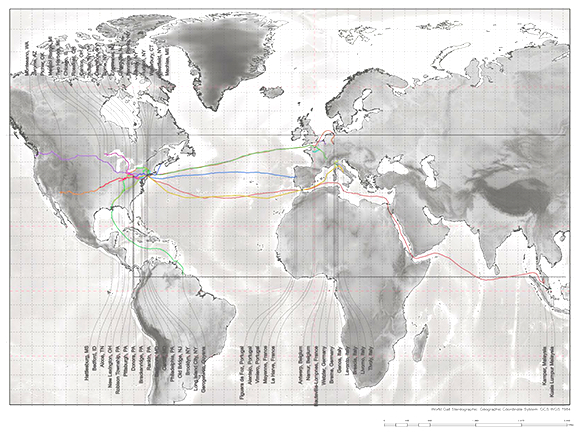
\includegraphics[width=1\linewidth]{figures/state.jpg}
    \caption{Provenance des matériaux et ressources nécessaires à la construction de l'Empire State Building en 1930. Carte réalisée en 2017 par Kiel Moe.}
    \label{fig:state}
\end{figure}
% Diaporama : conclusion de la séance 4 sans contenu, à compléter.
